\chapter{Fundamentals}
 Lorem ipsum dolor sit amet, consectetur adipiscing elit. Etiam in enim accumsan, egestas justo eget, venenatis velit. Duis gravida vehicula pharetra. Vivamus diam dolor, elementum dignissim varius eleifend, mattis in orci. Pellentesque elit justo, iaculis at suscipit eu, gravida at est. In hac habitasse platea dictumst. Integer in eleifend justo. Sed ornare, lorem at iaculis tristique, tellus odio pharetra arcu, in tempor lorem justo in ipsum. Nullam posuere tincidunt felis, vitae egestas dui fermentum sit amet. Phasellus elementum congue turpis, volutpat laoreet risus venenatis ac. Vivamus sed sapien diam.

Curabitur id fermentum nunc, in ornare magna. Nullam nibh mauris, lacinia sed leo vitae, porta egestas ex. Duis nisl risus, maximus eu sagittis vitae, rutrum imperdiet quam. Pellentesque felis nunc, rutrum vitae urna eget, feugiat eleifend erat. Nam congue enim et tellus laoreet, eu congue urna placerat. In pellentesque elementum luctus. Morbi ornare ac ipsum in sodales. Aenean eget porttitor urna, eget ultricies lectus. Nunc ac erat vitae turpis consectetur dictum et sed quam. Fusce cursus consectetur justo, sit amet feugiat velit vulputate eu. Nunc dolor sapien, posuere nec diam sit amet, suscipit aliquam justo. 
\begin{figure}[!h]
	\centering
    \def\svgwidth{0.5\textwidth}
%    \includestandalone[width=\textwidth]{figures/fig/lstmtikz}
    \input{figures/inkscape/aimldl.pdf_tex} %use full path to know the location of pdftex
    \caption{AIMLDL}
    \label{fig:ai_ml_dl}
\end{figure}

\begin{figure}[h]
	\begin{center}
	   \def\svgwidth{0.7\textwidth}
%    \includestandalone[width=\textwidth]{figures/fig/lstmtikz}
    \input{figures/inkscape/sigmoid.pdf_tex} %use full path to know the location of pdftex
	\end{center}
    \caption{Activation functions}
    \label{fig:activationfunctions}
\end{figure}

\begin{figure}[h]
	\begin{center}
	   \def\svgwidth{0.7\textwidth}
%    \includestandalone[width=\textwidth]{figures/fig/lstmtikz}
    \input{figures/inkscape/jaguarsensorconstellation.pdf_tex} %use full path to know the location of pdftex
	\end{center}
    \caption{AIMLDL}
    \label{fig:Sensors}
\end{figure}
\iffalse
\begin{figure}[h]
    \begin{center}
        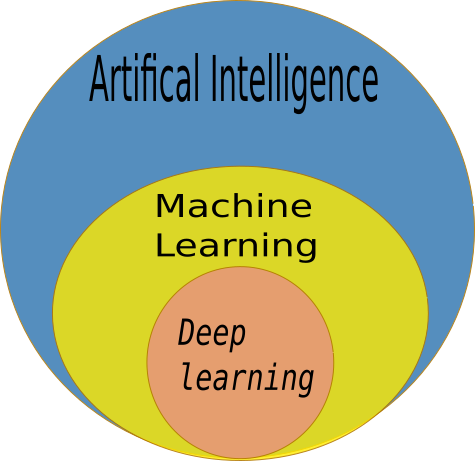
\includegraphics[width =0.3\textwidth]{figures/inkscape/aimldl.png}
    \end{center}
    \caption{Representing Artificial Intelligence, Machine Learning and Deep Learning as a
    subset of one another.}
    \label{fig:ai_ml_dl}
\end{figure}


\begin{figure}
	\centering
    \includestandalone[width=\textwidth]{figures/fig/multilayer_perceptron}
    \caption{Multilayer Perceptron.}
    \label{fig:multilayer_perceptron}
\end{figure}

\begin{figure}
	\centering
    \includestandalone[width=\textwidth]{figures/fig/SLsetup}
    \caption{Supervised Learning set up}
    \label{fig:SL_setup}
\end{figure}

\begin{figure}
	\centering
    \includestandalone[width=\textwidth]{figures/fig/2d_convolution}
    \caption{Two dimensional convolution}
    \label{fig:2dconv}
\end{figure}

\begin{figure}
	\centering
    \includestandalone[width=\textwidth]{figures/fig/dropout}
    \caption{Illustrating dropout functionality}
    \label{fig:Dropout_function}
\end{figure}

\fi

